\documentclass[sigchi]{acmart}
\usepackage{algorithm}
\usepackage[noend]{algpseudocode}
\usepackage{natbib}
\usepackage{quoting}
\usepackage{tikz}

\AtBeginDocument{%
  \providecommand\BibTeX{{%
    \normalfont B\kern-0.5em{\scshape i\kern-0.25em b}\kern-0.8em\TeX}}}

\settopmatter{printacmref=false, printccs=false, printfolios =false}
\setcopyright{none} 
\renewcommand\footnotetextcopyrightpermission[1]{}

\acmConference[MSA A.A. 2019-2020]{ }{September, 2020}{ }

\begin{document}

\title{Analysis of "Cloudlet-based Efficient Data Collection in Wireless Body Area Networks" report}

\author{Andrea Graziani}
\email{andrea.graziani93@outlook.it}
\affiliation{%
  \institution{Università Degli Studi di Roma Tor Vergata}
  \city{Rome}
  \state{Italy}
}

\renewcommand{\shortauthors}{Andrea Graziani (0273395)}

\maketitle

\section{Introduction}

\subsection{Research's Goal}

\vspace{0.3cm}

\begin{quoting}[font=itshape, begintext={``}, endtext={''\cite[par.~1.4]{MSAReport}}]
The main goal of this paper is to develop a large scale WBANs system in the presence of cloudlet-based data collection model. The objective is to minimize end-to-end packet cost by dynamically choosing data collection to the cloud by using cloudlet based system [...] reducing packet-to-cloud energy, the proposed work also attempt to minimize the end-to-end packet delay
\end{quoting}

\vspace{0.3cm}

According to \citet{MSAReport}, the goal of their work is to built an efficient \textbf{Wireless Body Area Networks} (\textbf{WBAN}) exploiting \textbf{edge computing}, a new paradigm in which substantial computing and storage resources, referred to as \textbf{cloudlets}, are placed at the Internet's edge, that is in close proximity to WBAN devices or sensors.\cite{TheEmergenceOfEdgeComputing}

To be more precise, as stated by \citet{MSAReport}, edge computing resources are exploited in order to \textbf{minimize average power consumption and delay} when \textbf{Personal Digital Assistant} (\textbf{PDA}) transmit collected data.

\subsection{Edge Computing Application Typology}

\vspace{0.3cm}

\begin{quoting}[font=itshape, begintext={``}, endtext={''\cite[par.~3.2]{MSAReport}}]
In our implementation, the enterprise cloud system will be the ultimate destination of the collected data. The enterprise cloud is also able to send messages back to both the cloudlet system or to WBAN users.
\end{quoting}

\vspace{0.3cm}

\begin{quoting}[font=itshape, begintext={``}, endtext={''\cite[par.~4.1]{MSAReport}}]
The enterprise cloud system is a centralized management and storage point that can be accessed by different organizations that are interested in a certain type of data. Another important feature of the cloudlet system is the ability of bidirectional communications between many WBANs users.
\end{quoting}

\vspace{0.3cm}

WBAN devices and sensors have very stringent constraints in term of CPU performance, storage resources and battery life.

to perform a wide range of healthcare, military and sport application, \textbf{Tier-1}, which represents "\textit{the cloud}" in today's parlance, plays a very important role in this kind of system: cloud resources are exploited to overcome WBAN devices constraints, since Tier-1 represents, in terms of archival preservation, the \textit{safest place to store data}, ensuring the long-term integrity and accessibility, and the \textit{main execution site to perform expensive computations}, thanks to its almost unlimited elasticity. 

However cloud resources exploitation isn't a panacea due to some negative consequence, as the increasing of network \textbf{round-trip times} (\textbf{RTT}) experienced by mobile users. 

Therefore, \citet{MSAReport} have built a system capable to exploit edge computing resources too, in order to offload compute-intensive operations at very low latency.\cite{TheSeminalRoleEdgeNativeApplications}\cite{TheEmergenceOfEdgeComputing}

To be more precise, WBAN system prototype modelled by \citet{MSAReport} is intended for \textit{edge-accelerated, cloud-native applications}. Why?

\begin{description}

\item[cloud-native] because, to overcome stringent constraints on battery, performance and storage of WBAN devices, cloud resources are exploited, through offloading techniques over a wireless network, \textbf{to execute critical task}; in other words, as stated also by \citet{MSAReport}, \textit{cloud is the primary execution site and it is essential to provide services to final users}.

\item[edge-accelerated] because the system exploits edge computing resources \textbf{only when available}. In that way, that system is capable to provide optimal performance, but \textit{edge resources represents a secondary execution site, that is they are optional to provide services}.

\end{description}

According to \citet{TheSeminalRoleEdgeNativeApplications}, it is shown that edge-accelerated, cloud-native applications can have a \textit{modest} advantages in term of \textit{response times}, \textit{battery life}, \textit{ingress bandwidth demand reduction}, \textit{privacy} and \textit{fallback services}\cite{TheSeminalRoleEdgeNativeApplications}\citep{TheEmergenceOfEdgeComputing}, but, as \citet{TheSeminalRoleEdgeNativeApplications} states, edge computing potentiality is not fully exploited due to central role assigned to cloud.

However, it is true that any edge-accelerated, cloud-native applications involves less investment risk, much less software development, and their markets are much larger since they \textit{can function acceptably even in the absence of edge computing}.

\subsection{Edge Computing Resources exploitation}

How edge computing resources are been exploited in order to improve, as stated by \citet{MSAReport}, average power consumption and delay during packet transmissions? 

\subsubsection{Using an energy-efficient communication technology}

First of all, is very important to precise that \citet{MSAReport} research is based on the observation that using WiFi technology a WBAN user will be able to transmit data packet to the cloud with \textbf{low power consumption}, \textbf{low delay} and mostly \textbf{no connection cost} compared with cellular technology; in fact, they wrote:

\vspace{0.3cm}

\begin{quoting}[font=itshape, begintext={``}, endtext={''\cite[par.~3.1]{MSAReport}}]
It was shown that, via WiFi, the transmission power of a data packet of size 46 Bytes will cost about 30 mw and with a delay of 0.045 ms. On the other hand, a longer transmission range cellular network connection (e.g. 3G and LTE) is capable of transmitting the data packet to the cloud from any location that is cover by cellular network, which is usually a wider geographic area compared with the WiFi. It was shown that, via cellular, the transmission power of data packet of size 46 Bytes will cost about 300 mw and with a delay of 0.45 ms.
\end{quoting}

\vspace{0.3cm}

Therefore, since WiFi technology is more energy-efficient than cellular technology, if WBAN users have the chance to use it, is possible to reduce average power consumption during packet transmission. 

However, how to exploit WiFi technology in WBAN system taking into account its \textbf{short transmission range} compared to cellular network? Providing an edge computing infrastructure made up of several cloudlets geographically distributed and equipped with computational, storage and communication capability, increasing WiFi coverage. In fact, researchers wrote:

\vspace{0.3cm}

\begin{quoting}[font=itshape, begintext={``}, endtext={''\cite[par.~4.1]{MSAReport}}]
The cloudlet system is composed of set of physical servers with many cores and huge Gigabytes of memory. The cloudlet server system is equipped with one or more of the communication antennas that is supporting different physical layer capabilities (e.g. WiFi and WiMax). 
\end{quoting}

\vspace{0.3cm}

However there is a problem: since WiFi technology transmission range is short and edge infrastructure resources are expensive,  cloudlet and WiFi coverage aren't available everywhere. Therefore, \citet{MSAReport} implemented a \textit{self-adaptive behaviour} according to which \textbf{communication technology is dynamically changed} when users move from one region to another. This is the reason according to which \citet{MSAReport} modelled their system identifying three different regions:\cite[par.~3.1]{MSAReport} 

\begin{description}

\item[Cloudlet Region (CR)] where WiFi coverage is available, so a user can use it to transmit data to the cloudlet.

\item[Enterprise Region (ER)] where only cellular coverage is available, therefore  a user can use only cellular technology to transmit a data packet to cloud. 

\item[Not-covered Region (NC)] where neither WiFi nor cellular technology is available. In this case a user should buffer the packets until one of the above technologies is available, then to be able of transmitting the packet to the enterprise cloud. 

\end{description}

In other words, WBAN users are capable to exploit edge computing resources if and only if they are in a \textit{Cloudlet Region}, otherwise they go on transmitting data directly to the cloud, if possible. This is the reason according to which we have previously defined \citet{MSAReport} application as \textit{edge-accelerated}: cloud is very critical for that application since it represents the ultimate destination of collected data and perform critical task providing access to data. In other words, seem enough clear that cloudlet is less critical compared to cloud to providing system services. In fact, \citet{MSAReport} wrote:

\vspace{0.3cm}

\begin{quoting}[font=itshape, begintext={``}, endtext={''\cite[par.~3.2]{MSAReport}}]
In our implementation, the enterprise cloud system will be the ultimate destination of the collected data. The enterprise cloud is also able to send messages back to both the cloudlet system or to WBAN users.
\end{quoting}

\vspace{0.3cm}

\begin{quoting}[font=itshape, begintext={``}, endtext={''\cite[par.~4.1]{MSAReport}}] 
The enterprise cloud system is a centralized management and storage point that can be accessed by different organizations that are interested in a certain type of data. 
\end{quoting}

\vspace{0.3cm}

\subsubsection{Exploiting network proximity}

Deploying cloudlet \textit{close} to final users, thanks to \textbf{high-bandwidth single-hop connection}, is possible to reduce RTT and to increase end-to-end bandwidth; in other words, we can achieve \textbf{network-proximity}.\citep{TheSeminalRoleEdgeNativeApplications}

However, is very important to not confuse \textit{physical proximity} with \textit{network-proximity}. Cloudlet physical proximity not always can affect positively RTT since it does \textit{not} guarantee network proximity: think for example to a highly congested WiFi network which may have poor RTT. Theoretically, is possible to achieve network proximity without physical proximity, for example using a fiber link between a wireless access point and a cloudlet that is many tens or even hundreds of kilometres away assuring therefore low RTT and high bandwidth.\cite{TheSeminalRoleEdgeNativeApplications}

\subsubsection{Using cyber-foraging techniques}

WBAN sensors and devices collect a very huge amount of data. In fact, \citet{MSAReport} wrote:

\vspace{0.3cm}

\begin{quoting}[font=itshape, begintext={``}, endtext={''\cite[par.~1.1]{MSAReport}}]
The multiple WBAN sensor nodes are capable of sampling, processing, and communicating one or more vital signs like heart rate, blood pressure, oxygen saturation, breathing rate, diabetes, body temperature, ECG and activity, or environmental parameters like location, temperature, humidity, light, movement, proximity and direction. 
\end{quoting}

\vspace{0.3cm}

Obliviously, WBAN devices and sensors cannot have enough computation and storage resources due to their very strictly constrains in term of size and power consumption. 

In order to overcome WBAN devices limitation, increasing energy efficiency, several cyber-foraging techniques are used: \citet{MSAReport} adopt a \textbf{Data Staging Tactic} to allow WBAN devices, after offloading collected data to cloudlet or cloud, to free up storage space. To achieve energy-efficiency, all computations regarding collected data are carried out by cloud or cloudlet, therefore \textbf{Computation Offload Tactic} is used too.

\citet{MSAReport} adopt a very static approach to offloading since, if a offload target is available, data will be \textit{always} offloaded. 
However, WBAN users devices exhibit a self-adaptive behaviour according to which they can decide to offload towards cloud instead of clodulet if Wifi network is highly congested; in fact, researchers wrote:

\vspace{0.3cm}

\begin{quoting}[font=itshape, begintext={``}, endtext={''\cite[par.~5.1]{MSAReport}}]
each VC region is able to serve a certain number of users [...] Then, the extra users within the VCs have to send the data via the cellular communication, even though, they are within the VCs. 
\end{quoting}

\vspace{0.3cm}

\subsection{A self-adaptive system}

It's clear that \citet{MSAReport} had built a \textbf{self-adaptive system} because it is capable to change its behaviour when execution environment changes. Let's now try to be more precise:

\begin{itemize}

\item From a deployment point of view, this system represents a \textbf{distributed self-adaptive system} since a self-adaptive software, including both \textit{managed software} and \textit{managing software}, is deployed in every WBAN users device.\cite{PatternsDecentralizedSelf}

\item From decisions control point of view, we can consider it a \textbf{decentralized self-adaptive system} too due to the lack of a central control component that decides about when and how to perform an adaptation; in other words, all WBAN nodes are responsible for adaptations, therefore control decision is decentralized.\cite{PatternsDecentralizedSelf} 

However, is very important to precise that in \citet{MSAReport} system there is no coordination between WBAN nodes referring to control decision. All  of them act independently, deciding adaptations autonomously, therefore, any kind of control decisions decentralization pattern is been used.  

\item From an architectural point of view, that system is based on a \textbf{MAPE-K feedback control loop} and represents a \textbf{autonomic system}. In fact, all WBAN nodes act as \textit{autonomic elements} because they manage their behaviour in accordance not only with execution environmental changes, but according to \textit{policies and goals} established by \citep{MSAReport} too. In other words, that system has \textbf{self-management capabilities}, relieving WBAN users of the responsibility of directly managing their device changing communication technology to achieve established goals; as known, self-management is the essence of autonomic computing.\cite{visionOf}

Let's study in deep the control feedback loop of that system:
\begin{description}

\item[Knowledge/Goal] The goals established by \citet{MSAReport} are average power consumption and average transmission delay minimization.

\item[Monitor] The monitoring process is responsible for collecting data from environment like network quality and WiFi or cellular connection availability. 

\item[Analyse] Measured data are analysed in order to detect WiFi congestion condition level ("Low" or "High") and check what is the current region ("NC", "ER" or "CR") where user is.

\item[Plan] Select and plan a solution to achieve established goal in according to system state diagram represented in \ref{fig:Chain}. 

\item[Execute] Change communication technology according to current state.

\end{description}

\item \citet{MSAReport} solution can be considered as \textbf{application-transparent} since WBAN applications are \textit{not} informed that a communication technology change is occurred; in other words, underlying system is the only responsible for the adaptation. In this way, compatibility with already existing applications is assured, although adaptations can affect negatively on WBAN applications. 

\end{itemize}

\begin{figure}
\caption{State diagram of communication technology used by WBAN devices} \label{fig:Chain}
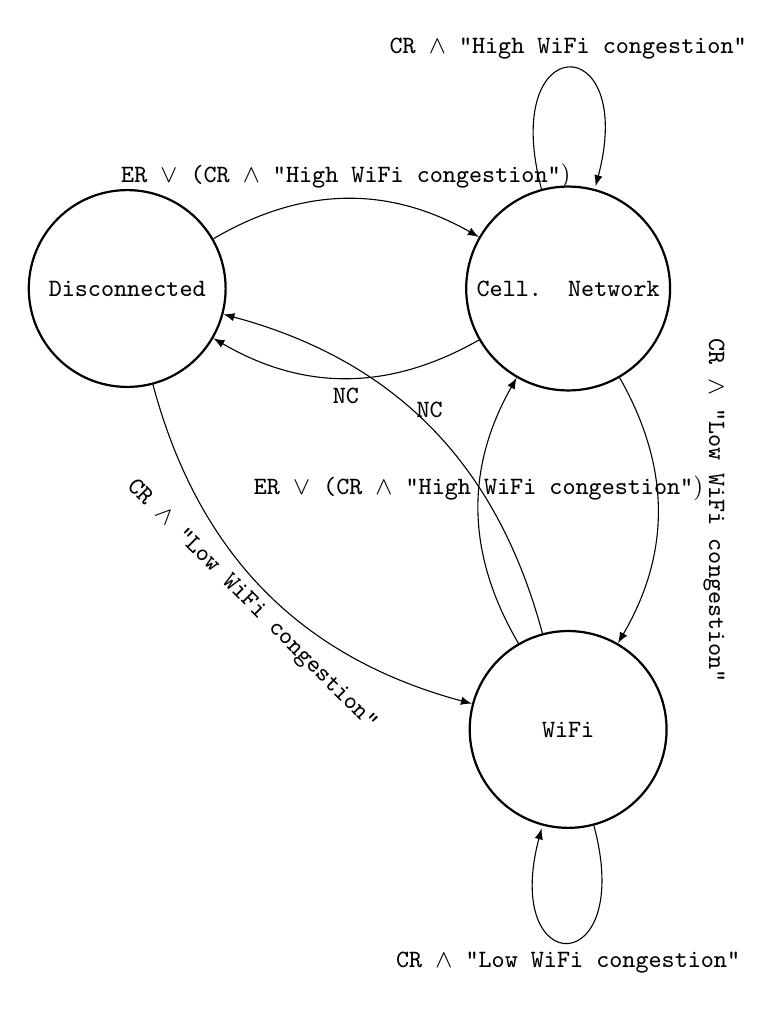
\begin{tikzpicture}[->,node distance=5.6cm,>=latex,font=\small, minimum width=2.5cm]

\tikzstyle{round}=[thick,draw=black,circle]

    \node[round] 			    		 (00) {\texttt{Disconnected}};
    \node[round,right of=00]      (10) {\texttt{Cell. Network}};
    \node[round,below of=10]    (01) {\texttt{WiFi}};

	\path 
 	(00) 	edge[bend left, above]        node	 	{\texttt{ER $\vee$ (CR $\wedge$ "High WiFi congestion"})} 							(10)
 	        edge[bend right, below]      node [rotate=-45]				    {\texttt{CR $\wedge$ "Low WiFi congestion"}} 							(01)
 	
	(10) edge[bend left, above]        node [xshift=13,rotate=-90]	{\texttt{CR $\wedge$ "Low WiFi congestion"}} 							(01)
		   edge[bend left, below]        node 	{\texttt{NC}} 																		(00)
		   edge[loop above]      		  node   {\texttt{CR $\wedge$ "High WiFi congestion"}} 							(10)
		   
	(01) edge[loop below]      		  node   {\texttt{CR $\wedge$ "Low WiFi congestion"}} 							(01)
		   edge[bend left, above]       	 node 	{\texttt{ER $\vee$ (CR $\wedge$ "High WiFi congestion"})} 						(10)
		edge[bend right, above]       	 node 	{\texttt{NC}} 						(00);

\end{tikzpicture}
\end{figure}

\subsection{Communication style}

Basically, when a device cannot transfer data packet to cloudlet for some reason, WBAN users are obliged to communicate directly with server-side application running on cloud, therefore a classical \textbf{client-server style communication} is adopted, which use classic \textit{point-to-point} and \textit{synchronous} communications. As known, use this kind of communication can be problematic due to \textbf{high degree of coupling between server and client}, like the lack of failure transparency or latency issue due to blocking nature of that kind of communication.

However, when a WBAN user is capable to communicate through a server, the system adopts another communication style: \textbf{server-side client/agent/server model}. In that case, the \textit{agent} is the cloudlet, which, acting as a surrogate to perform cyber-foraging tactics, is located on the so-called "\textit{fixed}" side portion of the network and, precisely, on the edge of the network. That \textbf{loose-connector} style is capable to reduce coupling degree between server and client achievement several advantages in term of failure transparency (cloudlet can mask temporary cloud application unavailability).

\section{Simulations Analysis}

In these section we will analyse simulation's results performed by \citet{MSAReport} in order to quantify performance advantages by using edge computing resources. 

WBAN system performance is evaluated through several simulation sets focusing mainly on two performance metrics:

\vspace{0.3cm}

\begin{quoting}[font=itshape, begintext={``}, endtext={''\cite[par.~4.2]{MSAReport}}]
\textit{Packet Transmission Power} and \textit{Packet Delay}. The Packet Transmission Power and Packet Delay are directly measure of the communication energy and delay expenditure from the Personal Digital Assistant (PDA) device to the cloudlet or the enterprise cloud
\end{quoting}

\vspace{0.3cm}

As stated by \citet{MSAReport}, experiments were carried out using a custom version of \textit{CloudSim}\footnote{\url{http://www.cloudbus.org/cloudsim/}} simulator, monitoring a virtual space-area, where several cloudlet entities were deployed in known geographic locations, in such a way transmission range belonging to different cloudlet not overlapping, while some WBAN users were moved randomly with fixed speed and random pause time.

\subsubsection{MAC protocol}

According to \citet{MSAReport}, the medium access mechanisms used in their simulation is \textbf{pooling-based}, that is a strictly centralized scheme, also called \textbf{point coordination function} (\textbf{PCF}), in which the access point, called \textbf{master}, dynamically polls clients for data. According to this scheme, the master is allowed to build a list of stations wishing to transmit during a contention phase. After this phase, the station polls each station on the list.

In a WBAN's context, this choice has several advantages:

\begin{itemize}

\item PCF is capable to offer time-bounded service, \textbf{guaranteeing a maximum access delay and minimum transmission bandwidth} making the system more \textbf{predictable} and, therefore, more suitable for \textbf{real-time} health monitoring; in fact, if a predictable system is used, will be possible to know with reasonable approximation the \textit{worst case execution time} (WCET) of jobs and check if any hard real-time constraints is respected.

\item Since WBAN users are not allowed to send data without the master's invitation, the \textbf{hidden terminal problem is eliminated}. Keep in mind that using DCF (Distributed coordination function) with RTS/CTS extension, in order to resolve hidden terminal problem, is not suitable in a WBAN's context because to short frame (only 46 byte) send by devices; RTS/CTS extension would introduce a non-negligible overhead causing a waste of bandwidth, higher delay and energy consumption.\cite{schiller2003mobile}

\item This scheme allow higher throughput due to less collisions respect to CSMA/CA.\cite{schiller2003mobile}

\end{itemize}

Obliviously this choice isn't a panacea; it can introduce higher delay under a light load and overhead if nodes have nothing to send.\cite{schiller2003mobile}

\subsection{First experiment set}

First experiment set goal is to quantify both \textbf{packet process delay} and \textbf{power consumption}, due to packet computation, by cloudlet varying following system parameter.

\begin{enumerate}

\item number of virtual machine deployed on a cloudlet (0, 2, 4 or 8). The maximum number of deployable virtual machines is bounded by the number of physical processors available on cloudlet (\citet{MSAReport} prototype cloudlet have 8 physical processors, therefore 8 is the maximum number of deployable VMs).
 
\item processing speed of data packet, from a minimum 100 to a maximum of 900 \textbf{million instructions per second} (MIPS).

\item number of WBAN users (up to 150 users).

\end{enumerate}

According to experiments results, \cite{MSAReport} have shown that:

\begin{enumerate}

\item Increasing the number of virtual machines running on a cloudlet, packet process delay will be reduced.

It is shown that, if data packets can be processed in \textbf{parallel}, the \textbf{blocked time} can be reduced. In fact, fixed data packet \textit{average arrival rate} $\lambda$ and \textit{average service rate} $\mu$ of each virtual machine, system cloudlet \textbf{utilization}, that is \textit{the fraction of time according to which cloudlet is busy}, is reduced; each virtual machine, by symmetry, sees an arrival rate of $\dfrac{\lambda}{k}$, where $k$ is the number of deployed virtual machines. Therefore cloudlet utilization, which is equal to $\dfrac{\lambda}{k\mu}$, decrease increasing $k$. According to the famous Erlang-C formula, decreasing utilization, \textbf{blocked time} is been reduced.

From an architectural point of view, the increase of the number of virtual machines on a cloudlet can be considered as a \textbf{performance tactic} and, precisely, a \textbf{resource management tactic}, because affects the time within which a response is generated with a better resources management achieved through concurrency.

\vspace{0.3cm}

\begin{quoting}[font=itshape, begintext={``}, endtext={''\cite[par.~3.3]{MSAReport}}]
the processing time is decreased by approximately 85\% by using cloudlet system configured with 8 VMs comparing to using only one VM in CS.
\end{quoting}

\vspace{0.3cm}

\item Fixed the average time required to process a packet data on a CPU, that is for a given MIPS process speed, power consumption and processing delay are increased by increasing the number of users. This happens because cloudlet utilization increases because $\lambda$ is higher, therefore the fraction of time according to which cloudlet is busy increases too; so, since more time is needed to complete user tasks, more power are consumed.

\end{enumerate}

\subsection{Second experiment set}

Second experiment set was carried out in order to quantify advantages of using edge computing resources. To be more precise, that simulation monitors the effects on \textbf{average transmission power and delay} of data packed send by users PDA to cloudlet, varying following system parameters:

\begin{enumerate}
\item number of cloudlet deployed (from 0 to 6).
\item WBAN user's positions (speed of $2\;m/s$ and a random pause time of $1-10\;s$)
\end{enumerate}

Monitored area size is fixed to $600 \times 400\;m$ while the total number of users is fixed to $400$.

According to experiments results, \cite{MSAReport} have shown that:

\begin{enumerate}

\item As expected, increasing the number of available cloudlets in monitored area, average transmission delay of data packed is reduced. It happens since the probability  that an user is close to one of them increases. Having more opportunities to transmit data within cloudlet coverage, users can benefit of cloudlet physical proximity which, as already said in previous section, \textit{can} decrease RTT, affecting positively latency, bandwidth and jitter. \cite{TheEmergenceOfEdgeComputing}. 

As known, when cloudlet coverage is available, data is offloaded to a cloudlet using a high bandwidth single-hop connection, which decrease RTT. Conversely, when cloudlet coverage isn't available, data is offloaded to cloud using a \textbf{multi-hop network connections} which involves high RTT and likely low bandwidth connection.\cite{ArchitecturalTacticsCyberForaging}

\item Increasing the number of available cloudlets, average transmission power of data packed is reduced too. It is due to the use of WiFi technology which is, as already said, more energy-efficient compared to cellular network.

\item Increasing the number of users, both average transmission power and delay increase. This happens because:

\begin{enumerate}
\item When a cloudlet area contains a large number of users, interferences increase, leading to higher error bit rate and affecting negatively both transmission delay, due to data packets or acknowledgements loss, and power, due to packet retransmission.

\item Since a polling MAC scheme is used, an higher number of users within an cloudlet WiFi coverage area increases the time needed to pool every node by AP. 

\item As stated by \citet{MSAReport}, an high congested WiFi network can cause WBAN devices to perform a self-adaptation action according to which communication technology is switched, using cellular network to send packet data instead WiFi, affecting negatively aforementioned metrics.
\end{enumerate}

\end{enumerate}

\subsection{Third experiment set}

The last experiment set is focusing on monitoring aforementioned performance metric varying cloudlet geographical placement. Monitoring an $800 \times 800 \; m$ area, simulations were carried out varying following system parameters:

\begin{enumerate}
\item number of cloudlet deployed (up to 16 cloudlets).
\item number of WBAN users (up to 1400 users).
\item WBAN user's positions (same parameters as before)
\item cloudlet geographical placement (using very different patterns, classified in three categories by \citet{MSAReport}: \textit{Adjacent}, \textit{Distant} and \textit{Intermediate})
\end{enumerate}

Experiments results are the following:

\begin{enumerate}

\item As expected, independently from cloudlet deployment pattern, increasing the number of cloudlet, the impact of cloudlet geographical placement on average transmission power and delay is negligible since, in that way, the opportunities to send the data packet to a cloudlet, using WiFi and with minimum cost of power and delay, increase.

\item Fixed cloudlet and users number, deploying cloudlet using an intermediate category pattern, that is placing cloudlet neither too far apart nor too close, system performance are better than other patterns belonging to other categories.

\end{enumerate}

\section{Further architectural considerations, issues and possible improvements}

\subsection{The cloudlet discovery and provisioning issue}

As said in previous section, \citet{MSAReport} overcome to WBAN devices limits, in term of computing power and storage, through cyber-foraging techniques like computation offload and data staging. We believe that the system model built by \citet{MSAReport} is too simple to achieve research's goals.

It is shown \cite{DecisionModel} that cyber-foraging systems have \textit{at a minimum} the following combination of functional requirements:

\begin{itemize}

\item  A need for computation offload, data staging, or both
\item  A need to provision a surrogate with the offloaded computation or data staging capabilities
\item  A need for the mobile device to locate a surrogate at runtime

\end{itemize}

Although WBAN users \textit{need} to be able to locate available cloudlet in an area where stage data, \textbf{cloudlet discovery} issue has \textit{not} been addressed by \citet{MSAReport} in any way; we believe that it is a very big mistake because cloudlet discovery affects negatively energy consumptions and response time and, anyway, it is a \textbf{functional requirements} for any cyber-foraging systems. 

However there is another reason which that makes cloudlet discovery issue so important: \textbf{security}. \citep{MSAReport} wrote:

\vspace{0.3cm}

\begin{quoting}[font=itshape, begintext={``}, endtext={''\cite[par.~3.3]{MSAReport}}]
On the other hand, since WBANs forward useful and life-critical information to the cloud, which may operate in distributed and hostile environments, novel security mechanisms are required to prevent malicious interactions to the storage infrastructure. Both the cloud providers and the users must take strong security measures to protect the storage infrastructure.
\end{quoting}

\vspace{0.3cm}

\citet{MSAReport} should have known that addressing cloudlet discovery issue, they could have improved system security. For example, using \textbf{Cloud Surrogate Directory} tactic, according to which mobile device contacts a cloud server that maintains a list of potential cloudlet/surrogates, security is highly increased because the mobile device only needs to trust the cloud surrogate directory server and can pre-exchange credentials for authorization. 

Generally, when you want to offload data or computation to a cloudlet, a selection algorithm to select best cloudlet is run. In WBAN systems, maximize energy efficiency, in order to preserve devices lifetime, is critical, therefore is preferable not run selection algorithm on WBAN devices, which can decrease energy efficiency (depending on the complexity of the algorithm and the number of monitored variables). Probably, using cloud surrogate directory tactic, according to which selection algorithms run on the cloud, is possible to improve WBAN lifetime. \cite{DecisionModel}

In the same way, \textbf{surrogate provisioning} is another functional requirements for any cyber-foraging systems which is not addressed by \citep{MSAReport}, therefore is not clear how cloudlets manage offloaded computation and/or data processing operations.

During the first experiment set, \citet{MSAReport} had shown that packet process delay is affected by the number of virtual machine deployed in cloudlet. However, provisioning tactic affects this process delay too. It is shown that Pre-provisioned cloudlet have the advantage of shorter provisioning times because the capabilities already reside on cloudlet, providing shorter response times to requests from mobile devices.\cite{DecisionModel}

\subsection{IEEE 802.11ah as communication standard}

In addition to changing communication technology, we believe that the use of a communication standard capable to minimize the dominant sources of energy waste like \textit{collision}, \textit{inter-network interference} between nearby WBAN devices, \textit{idle listening} and \textit{control packet overhead} is extremely useful to maximizing the lifetime of WBAN devices.

Unfortunately, \citet{MSAReport} give us very few details about MAC protocol according to which PDA send aggregated data packet to cloudlet. Not even specifying the version of the standard IEEE 802.11 used in their simulations, all we know is that \citep{MSAReport} use IEEE 802.11 with a pooling-based scheme and that WiFi transmission range not exceed 100 m in outdoor. In any case, based on what has been declared by \citep{MSAReport}, is reasonable to assume that they have used legacy IEEE 802.11 protocol with $2.4$ or $5$ GHz bands.

We believe that we can achieve better communication performances over longer distances among a large number of low-power devices exploiting \textbf{IEEE 802.11ah}. In fact:

\begin{itemize}
\item The 802.11ah standard enables single-hop communication over distances up to $1000$ m, utilizing sub-1 GHz license-exempt bands to provide better propagation characteristics in outdoor scenarios, like WBAN, than legacy WiFi. On the other side

\item IEEE 802.11ah MAC layer improves power efficiency through frame shortening techniques, reducing overhead caused by short packets transmission which are very common in WBAN scenario.

\item Several innovative concepts such as hierarchical \textit{Association IDentification} (AID), \textit{Restricted Access Window} (RAW), \textit{Group Sectorization} (GS), decrease collision probability in networks with thousands of stations, resolve hidden terminal problems, support a large number of associated stations, improving scalability and power efficiency.

\end{itemize}

\subsection{Resource demand tactics}

In addiction to edge computing resources exploitation, there is another performance tactic capable to reduce latency suitable for WBAN. In previous section, \citet{MSAReport} simulation results had shown that increasing the number of users within a cloudlet region affects negatively system performance for several reasons already explained. 

In order to reduce system utilization and so average packet process delay too, we can adopt a performance tactic according to which \textit{the number of packet to process is reduce managing the packets data generation rate}. In other words, if it is possible to reduce the sampling frequency at which environmental and body variables are monitored, demand can be reduced. A best approach could be to implement a self-adaptive behaviour according to which sampling frequency can varying according to users population within a cloudlet region or other system parameters, like network conditions o residual battery life. 

\subsection{Variable data fidelity tactic}

Unfortunately \citet{MSAReport} \textit{didn't introduce any variable data fidelity tactic} capable to improve WBAN battery life. We believe that the introduction of an \textbf{approximate computing} (and \textbf{storage}) technique can be useful in WBAN context. 

As known, approximate computing is a new paradigm based on the intuitive observation that, while performing exact computation require high amount of resources, allowing selective approximation or imperfect computations results can provide drastic energy savings.

To be more precise, approximate computing leverage the presence of error-tolerant code regions in applications and perceptual limitations of users to intelligently trade off implementation, storage and/or result accuracy for performance or energy gains. In brief, approximate computing exploits the gap between the level of accuracy required by the applications/users and that provided by the computing system.

For example, can be useful, in order to improve energy-efficiency, to reduce data fidelity collected by WBAN devices according to network condition, current position or battery status. For instance, we can adopt a technique according to which, when network condition are very bad or totally absent, in order to reduce the energy cost due to data buffering, critical application data (for example vital signs like heart rate, blood pressure, oxygen etc.) are stored in reliable memory segments with higher refresh rate, conversely less critical data (for example experimental data like location, temperature, humidity, light etc.) are stored into less reliable memory with a less refresh rate. As known, higher is refresh rate, higher is power consumption.\cite{Towards}

\citet{ApproximateComputingArticle} had shown that, using approximate computing techniques, applications run 3.78 times faster while energy consumptions are reduced 2.77 times. \citet{ImpactApproximation} achieve similar results, claiming that approximate computing can show up to 30\% energy savings.

\subsection{Scalability and elasticity tactic}

Solution proposed by \citep{MSAReport} doesn't exploit any scalability/elasticity tactic in order to increase cloudlet resource efficiency achieving scalability and elasticity. Keep running several virtual machines on a cloudlet while there are few WBAN users within a cloudlet region is a real waste of resources. Moreover full virtualization approaches are usually unsuitable for deploying distributed applications due to their overhead and long boot time.

OS-level virtualization based tools, also called \textbf{containers}, are often a better choice for scalability and elasticity purposes since they represent a lightweight alternative to virtual machine thanks to their very small footprint and quick boot time. 

Exploiting container advantages and using a scalability/elasticity tactic like \textbf{Just-in-Time containers tactic}, typically used to complement the computation offload tactic and data staging tactics, we can achieve aforementioned objectives. This tactic, in order to decrease the load on a cloudlet, supporting a greater number of requests, creates an instance of the offloaded code upon receipt of an offload request, destroying it when request is fulfilled. However, because the instance is created at runtime, there is a response/execution time penalty to create the instance before computation can execute.

\subsection{Mobility issue}

\citet{MSAReport} don't specify which transportation protocol is been used in their simulations and, once again, we believe that the lack of that information could be a problem because it is shown that transportation protocol has negative effects on performance in wireless communications, where many data packet can be lost due both to an \textit{high error bit rate} and to an \textit{high amount of disconnections} due to user mobility. For instance, TCP interpreters packet loss as a congestion symptom and the activation of its congestion control mechanisms can, as known, negatively affect performance. 

Since WBAN user can move from a region to another, several hand-offs can occur, causing data packets loss and performance worsening. Unfortunately, any information is given about \textit{average residence time} within a region by a WBAN user and the amount of hand-off performed during simulations. According to \citet{MSAReport}, WiFi coverage is limited to 100 m, very little if compared to cellular network transmission range. We believe that this situation could potentially lead to frequent hand-off and low residence time affecting negativity real applications.

\citet{MSAReport} doesn't report how \textit{users movements speed} (fixed to $2 m/s$) and the \textit{random pause time} (fixed to $1-10 s$) affected simulation's results and is not clear how they are intercorrelated with average power consumption and delay during the second and the third experiment set. Obliviously, we will expect that user speed is correlated to the amount of hand-off, therefore faster users involve more hand-offs, however this aspect was not considered. Moreover, we believe that \textbf{cloudlet region size} is a very important parameter since smaller cloudlet regions can potentially increase the amount of hand-off performed by an user. This aspect was also not considered.

Maybe, a better analysis regarding about aforementioned aspects could be very useful for real application and an \textbf{specification model} capable to highlight system state variable and equations and logic describing how the state variables are interrelated, including algorithms for computing their interaction and evolution in time, could be very useful to reproduce simulation and validate \citep{MSAReport} results.

\bibliographystyle{ACM-Reference-Format}
\bibliography{Bibliography}

\appendix

\end{document}
\endinput
